\documentclass[9pt,twocolumn,twoside]{pnas-new}
% Use the lineno option to display guide line numbers if required.

\articletype{CLASSIFICATION}%%%% Article topic/classification

\templatetype{pnasresearcharticle} % Choose template
% {pnasresearcharticle} = Template for a two-column research article
% {pnasmathematics} %= Template for a one-column mathematics article
% {pnasinvited} %= Template for a PNAS invited submission


\begin{document}


\title{Template for preparing your research report submission to PNAS using Overleaf}

% Use letters for affiliations, numbers to show equal authorship (if applicable) and to indicate the corresponding author
\author[a,c,1]{Author One}
\author[b,1,2]{Author Two}
\author[a]{Author Three}

\affil[a]{Affiliation One}
\affil[b]{Affiliation Two}
\affil[c]{Affiliation Three}

% Please give the surname of the lead author for the running footer
\leadauthor{Lead author last name}

% Please add a significance statement to explain the relevance of your work
\significancestatement{Authors must submit a significance statement between 50 and 120 words in length about the significance of their research paper written at a level understandable to an undergraduate educated scientist outside their field of speciality. The primary goal of the significance statement is to explain the relevance of the work in broad context to a broad readership. If submitting a Direct Submission, please add a significance statement to explain the relevance of your work. Brief Reports do not publish with a significance statement, and should be omitted for this article type.}

% Please include corresponding author, author contribution and author declaration information
\authorcontributions{Please provide details of author contributions here.}
\authordeclaration{Please declare any competing interests here.}
\equalauthors{\textsuperscript{1}A.O.(Author One) contributed equally to this work with A.T. (Author Two) (remove if not applicable).}
\correspondingauthor{\textsuperscript{2}To whom correspondence should be addressed. E-mail: author.two\@email.com}

% At least three keywords are required at submission. Please provide three to five keywords, separated by the pipe symbol.
\keywords{Keyword 1 $|$ Keyword 2 $|$ Keyword 3 $|$ ...}

\begin{abstract}
Please provide an abstract of no more than 250 words in a single paragraph. Abstracts should explain to the general reader the major contributions of the article. References in the abstract must be cited in full within the abstract itself and cited in the text.
\end{abstract}

\dates{This manuscript was compiled on \today}
\doi{\url{www.pnas.org/cgi/doi/10.1073/pnas.XXXXXXXXXX}}


\maketitle
\thispagestyle{firststyle}
\ifthenelse{\boolean{shortarticle}}{\ifthenelse{\boolean{singlecolumn}}{\abscontentformatted}{\abscontent}}{}

\Firstpage

%The \Firstpage command is used to format the first page text column size. The same size will be maintained for subsequent paragraph until the \Endparasplit or \Parasplit command is encountered.

This PNAS journal template is provided to help you write your work in the correct journal format. Instructions for use are provided below.

Note: please start your introduction without including the word ``Introduction'' as a section heading (except for math articles in the Physical Sciences section); this heading is implied in the first paragraphs.

\section*{Guide to using this template on Overleaf}

Please note that whilst this template provides a preview of the typeset manuscript for submission, to help in this preparation, it will not necessarily be the final publication layout. For more detailed information please see the  \href{https://www.pnas.org/author-center/submitting-your-manuscript}{PNAS Author Center}.


If you have a question while using this template on Overleaf, please use the Menu on the top bar and access the Documentation for \href{https://www.overleaf.com/help}{help and tutorials}. You can also \href{https://www.overleaf.com/contact}{contact the Overleaf support team} at any time with specific questions.

\subsection*{Author Affiliations}

For each author, include institutional unit (e.g., division, department, or section), institution, city, state with ZIP code (for US institutions) or country with postal code (for non-US institutions). Use lower case letters to match authors with institutions, as shown in the example. PNAS requires the corresponding author to provide an ORCID identifier at submission and strongly encourages all authors to use an ORCID ID. Do not include ORCIDs in the manuscript file; individual authors must link their ORCID account to their PNAS profile at \href{http://www.pnascentral.org/}{www.pnascentral.org}. For proper authentication, authors must provide their ORCID at submission and are not permitted to add ORCIDs on proofs.

\subsection*{Submitting Manuscripts}

All authors must submit their articles at \href{http://www.pnascentral.org/cgi-bin/main.plex}{PNAScentral}. If you are using Overleaf to write your article, you can use the ``Submit to PNAS'' option in the top bar of the editor window.

\subsection*{Format}

Many authors find it useful to organize their manuscripts with the following order of sections: introduction, results, discussion, materials and methods, acknowledgments, and references. Other orders and headings are permitted.

\subsection*{Manuscript Length}

A standard 6-page article is approximately 4,000 words, 50 references, and 4 medium-size graphical elements (i.e., figures and tables). The preferred length of Direct Submission articles remains at 6 pages, but PNAS will allow articles up to a maximum of 12 pages. Brief Reports are limited to 3 pages, which is approximately 1,600 words (including the manuscript text, title page, abstract, and figure legends), and 15 references.

\subsection*{References}

References should be cited in numerical order as they appear in text; this will be done automatically via bibtex, e.g. \cite{belkin2002using} and \cite{berard1994embedding,coifman2005geometric,phdthesis,masterthesis}. All references cited in the main text should be included in the main manuscript file.\Endparasplit

%The \Endparasplit command is used to end the formatting of the text column size that was set by the \Firstpage command. This will restore the default column size for the subsequent text.
%
%The \Parasplit command should be used if the page ends in the middle of a paragraph, allowing the column formatting to continue seamlessly on the next page.


\subsection*{Language-Editing Services}
Prior to submission, authors who believe their manuscripts would benefit from professional editing are encouraged to use a language-editing service (see list at https://www.pnas.org/author-center/language-editing). PNAS does not take responsibility for or endorse these services, and their use has no bearing on acceptance of a manuscript for publication.


\begin{figure}%[tbhp]
\centering
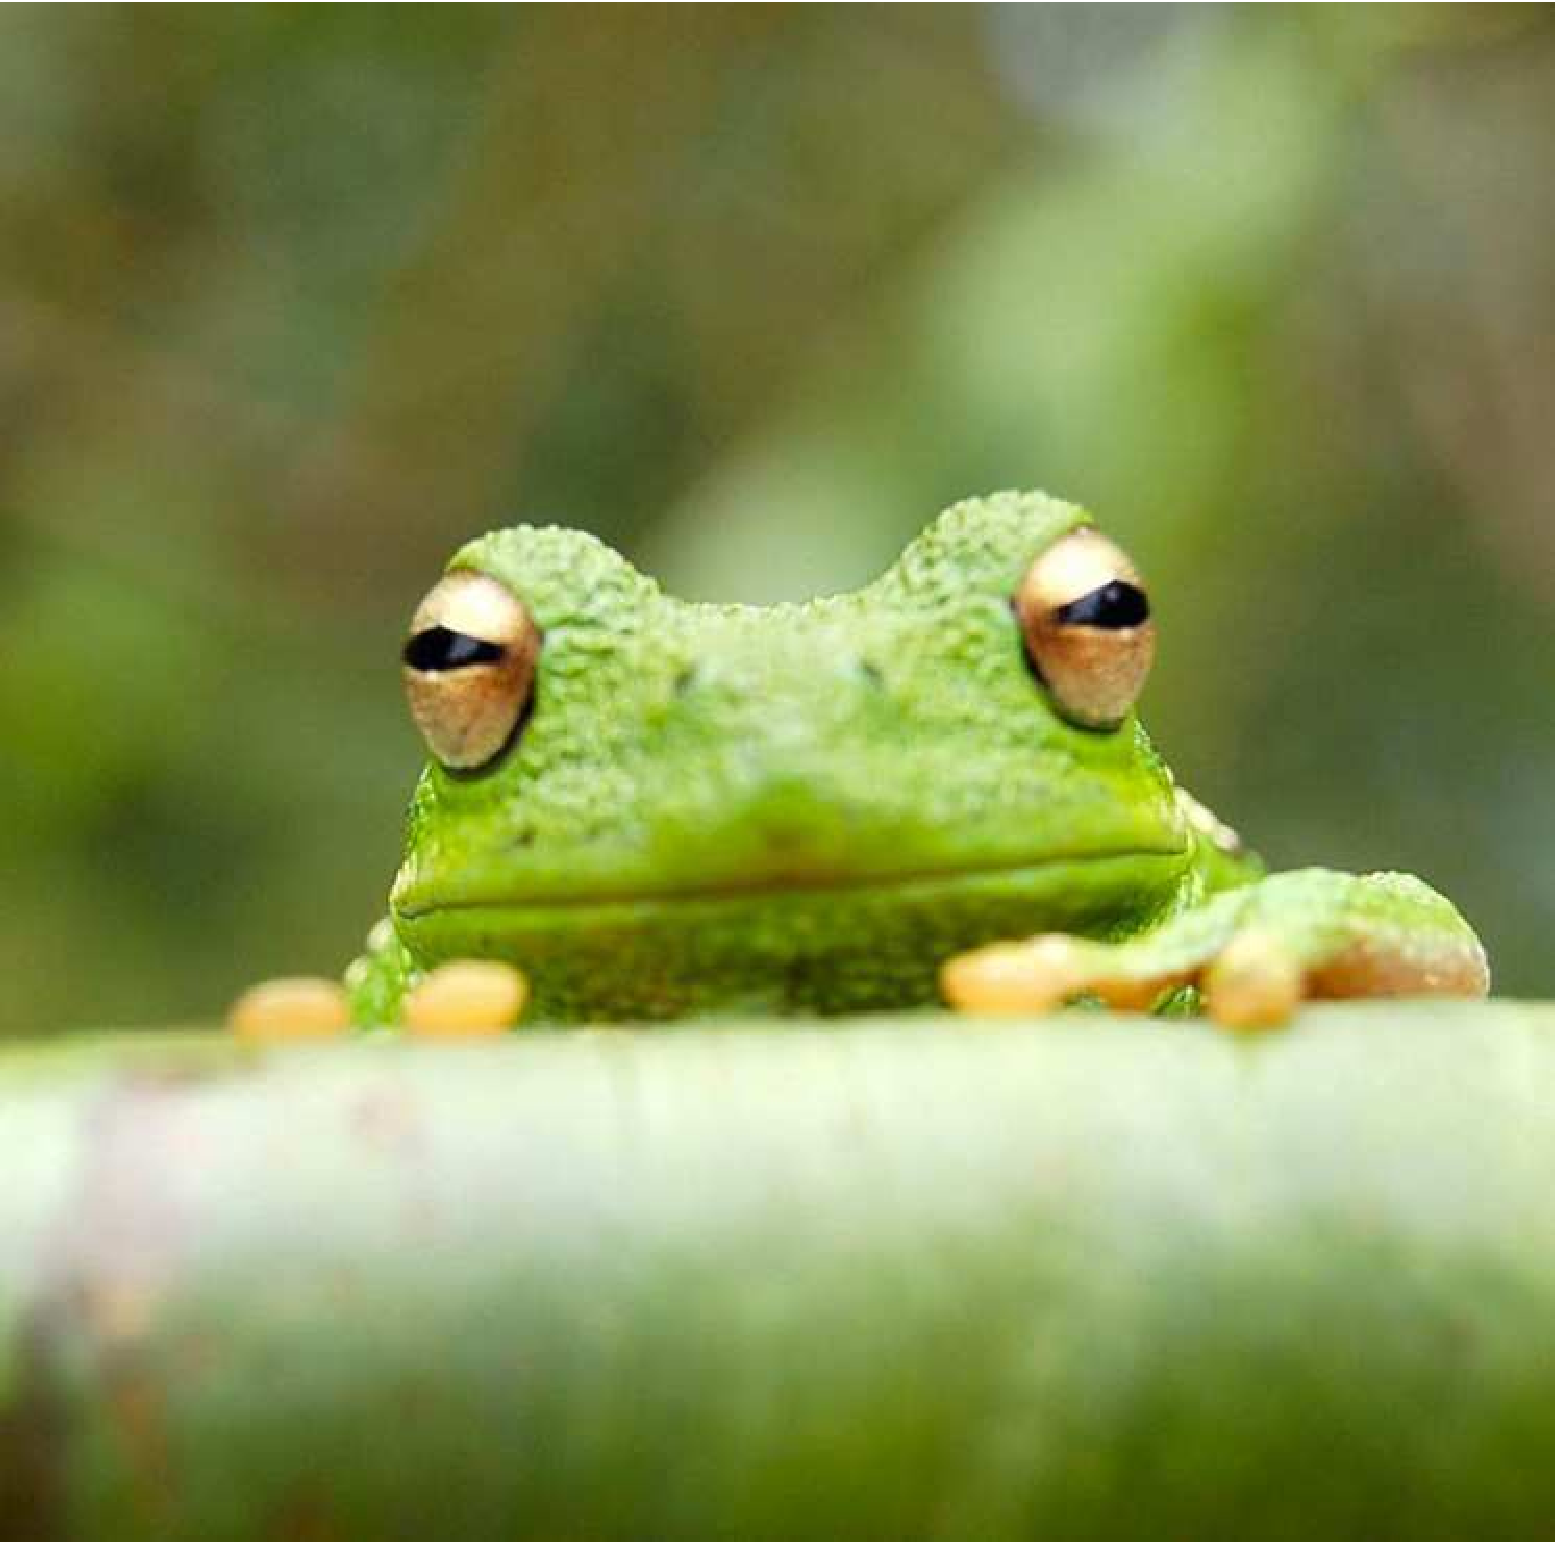
\includegraphics[width=.8\linewidth]{frog.pdf}
\caption{Placeholder image of a frog with a long example legend to show justification setting.}
\label{fig:frog1}
\end{figure}


\begin{figure*}[t!]
\centering
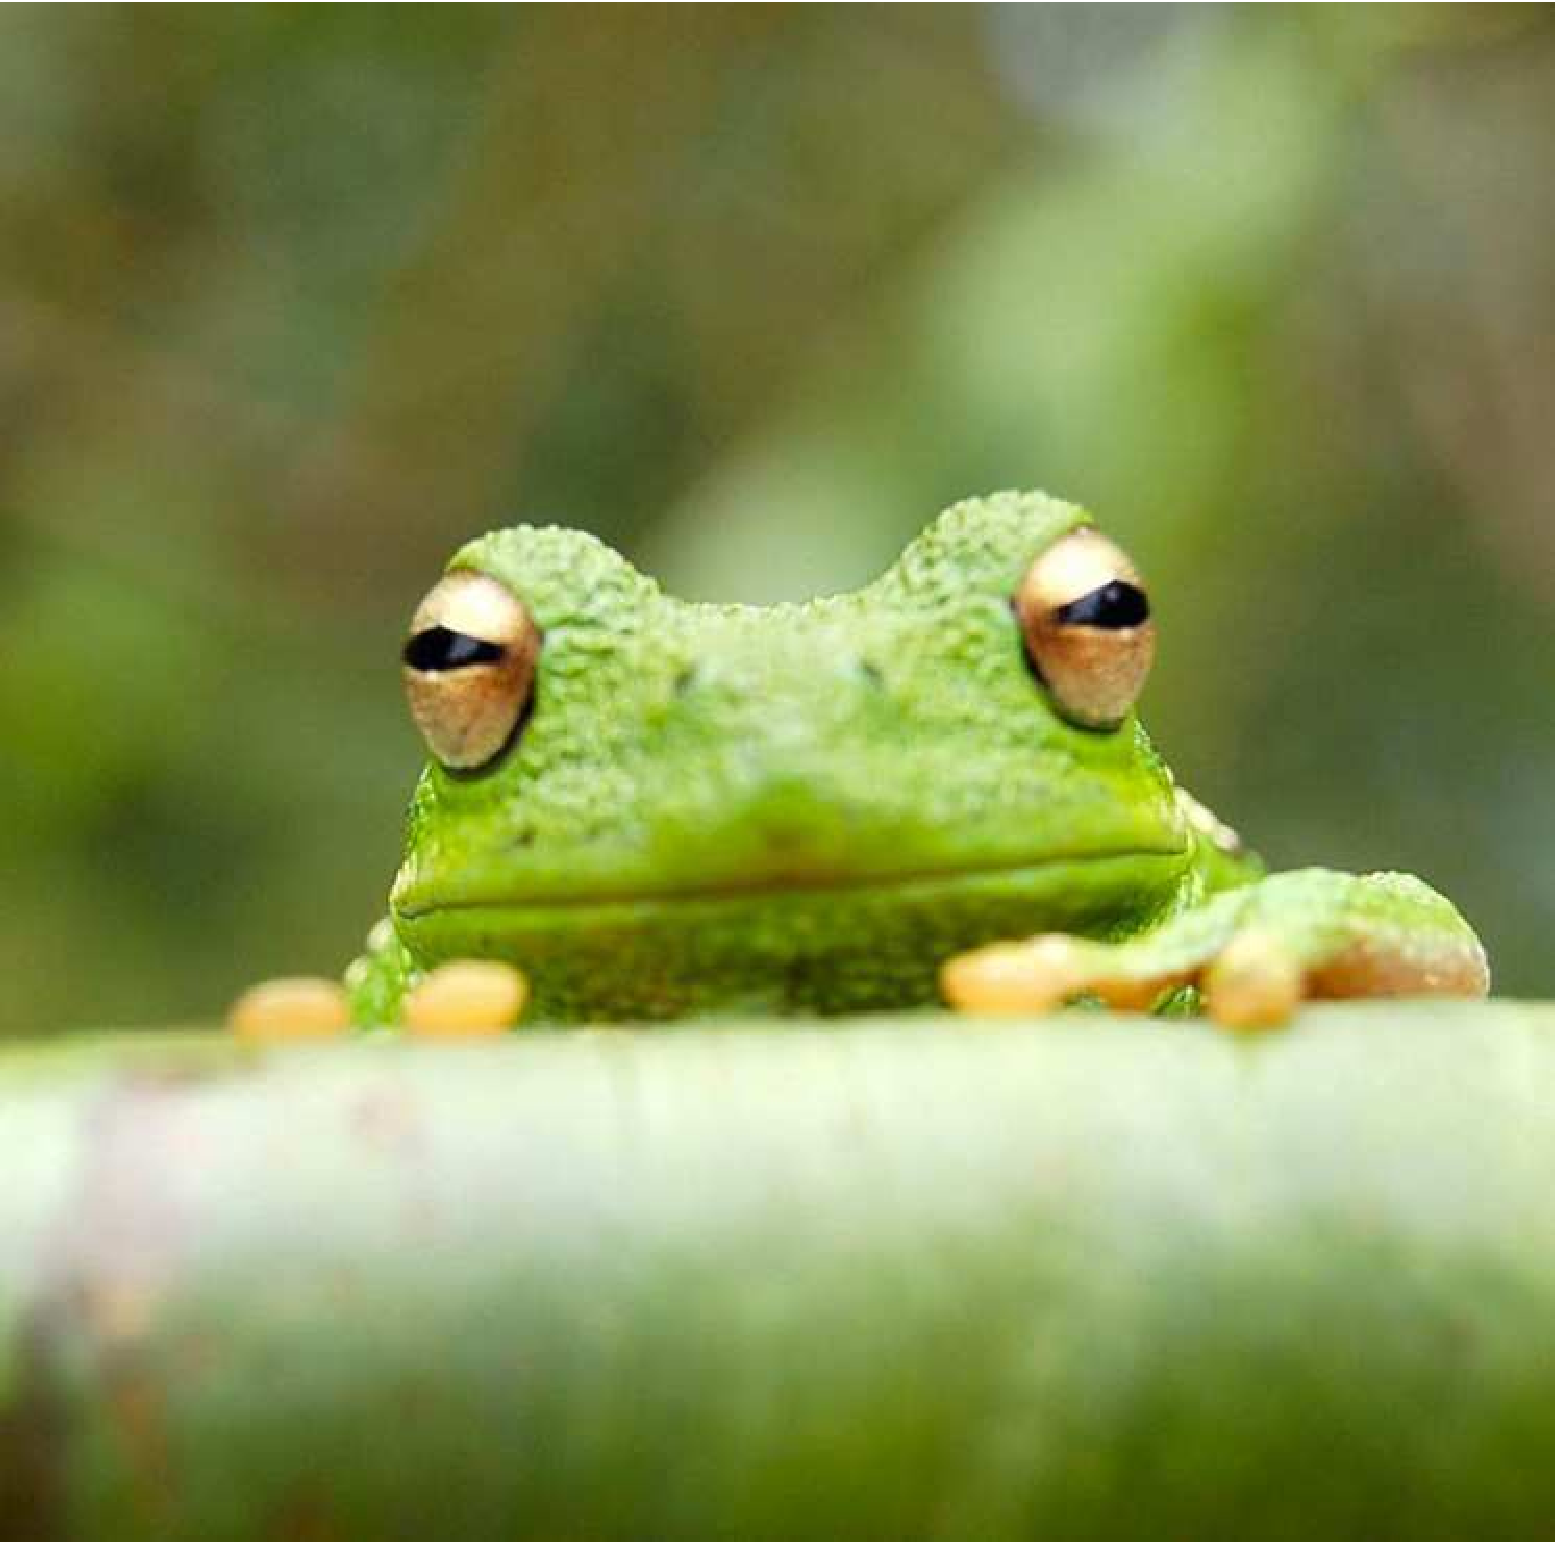
\includegraphics[scale=0.6]{frog}
\caption{Placeholder image of a frog with a long example legend to show justification setting.}
\label{fig:frog2}
\end{figure*}


\begin{table}[t!]
\centering
\caption{Comparison of the fitted potential energy surfaces and ab initio benchmark electronic energy calculations}
\begin{tabular}{lrrr}
Species & CBS & CV & G3 \\
\midrule
1. Acetaldehyde & 0.0 & 0.0 & 0.0 \\
2. Vinyl alcohol & 9.1 & 9.6 & 13.5 \\
3. Hydroxyethylidene & 50.8 & 51.2 & 54.0\\
\bottomrule
\end{tabular}

\addtabletext{nomenclature for the TSs refers to the numbered species in the table.}
\end{table}


\begin{table*}[t!]
\centering
\caption{Impact on Emission Behaviors by Socioeconomic Status}
\begin{tabular*}{\textwidth}{@{\extracolsep{\fill}}lccccc@{}}
& (1) & (2) & (3) & (4) & (5) \\
\midrule
 & \multicolumn{2}{c}{City-level} & Firm-level & \multicolumn{2}{c}{City-level} \\
Dep. Var.: & \multicolumn{2}{c}{COD Emission (1,000 tons)} & COD Emission (ton) & Firm Entry & Firm Exit \\
\multicolumn{6}{c}{Panel A: Population Share without College Education} \\
Share of Below College $\times$ Post$_{05}$ & 0.165*** & 0.292** & 0.358*** & 0.623** & 0.280 \\
 & (0.026) & (0.119) & (0.106) & (0.266) & (0.487) \\
Share of Below College & -0.208 & & & & \\
 & (0.141) & & & & \\
Post$_{05}$ & -16.426*** & & & & \\
 & (2.873) & & & & \\
\multicolumn{6}{c}{Panel B: Population Share without High School Education} \\
Share of Below HS $\times$ Post$_{05}$ & 0.099*** & 0.218** & 0.232** & 0.453** & 0.089 \\
 & (0.005) & (0.090) & (0.079) & (0.195) & (0.333) \\
Share of Below HS & -0.213* & & & & \\
 & (0.100) & & & & \\
Post$_{05}$ & -9.465*** & & & & \\
 & (0.564) & & & & \\
\bottomrule
\end{tabular*}

\addtabletext{*** P $<$ 0.01, ** P $<$ 0.05, * P $<$ 0.1}
\end{table*}

\subsection*{Digital Figures}

EPS and high-resolution PDF are preferred formats for figures that will be used in the main manuscript. Authors may submit PRC or U3D files for 3D images; these must be accompanied by 2D representations in TIFF, EPS, or high-resolution PDF format. Color images must be in RGB (red, green, blue) mode. Include the font files for any text.

Images must be provided at final size, preferably 1 column width (8.7cm). Figures wider than 1 column should be sized to 11.4cm or 17.8cm wide. Numbers, letters, and symbols should be no smaller than 6 points (2mm) and no larger than 12 points (6mm) after reduction and must be consistent.

Figures and tables should be labelled and referenced in the standard way using the \verb|\label{}| and \verb|\ref{}| commands.

Figure \ref{fig:frog1} shows an example of how to insert a column-wide figure. To insert a figure wider than one column, please use the \verb|\begin{figure*}...\end{figure*}| environment. Figures wider than one column should be sized to 11.4 cm or 17.8 cm wide. Use \verb|\begin{SCfigure*}...\end{SCfigure*}| for a wide figure with side legends.

\begin{SCfigure*}[\sidecaptionrelwidth][t!]
\centering
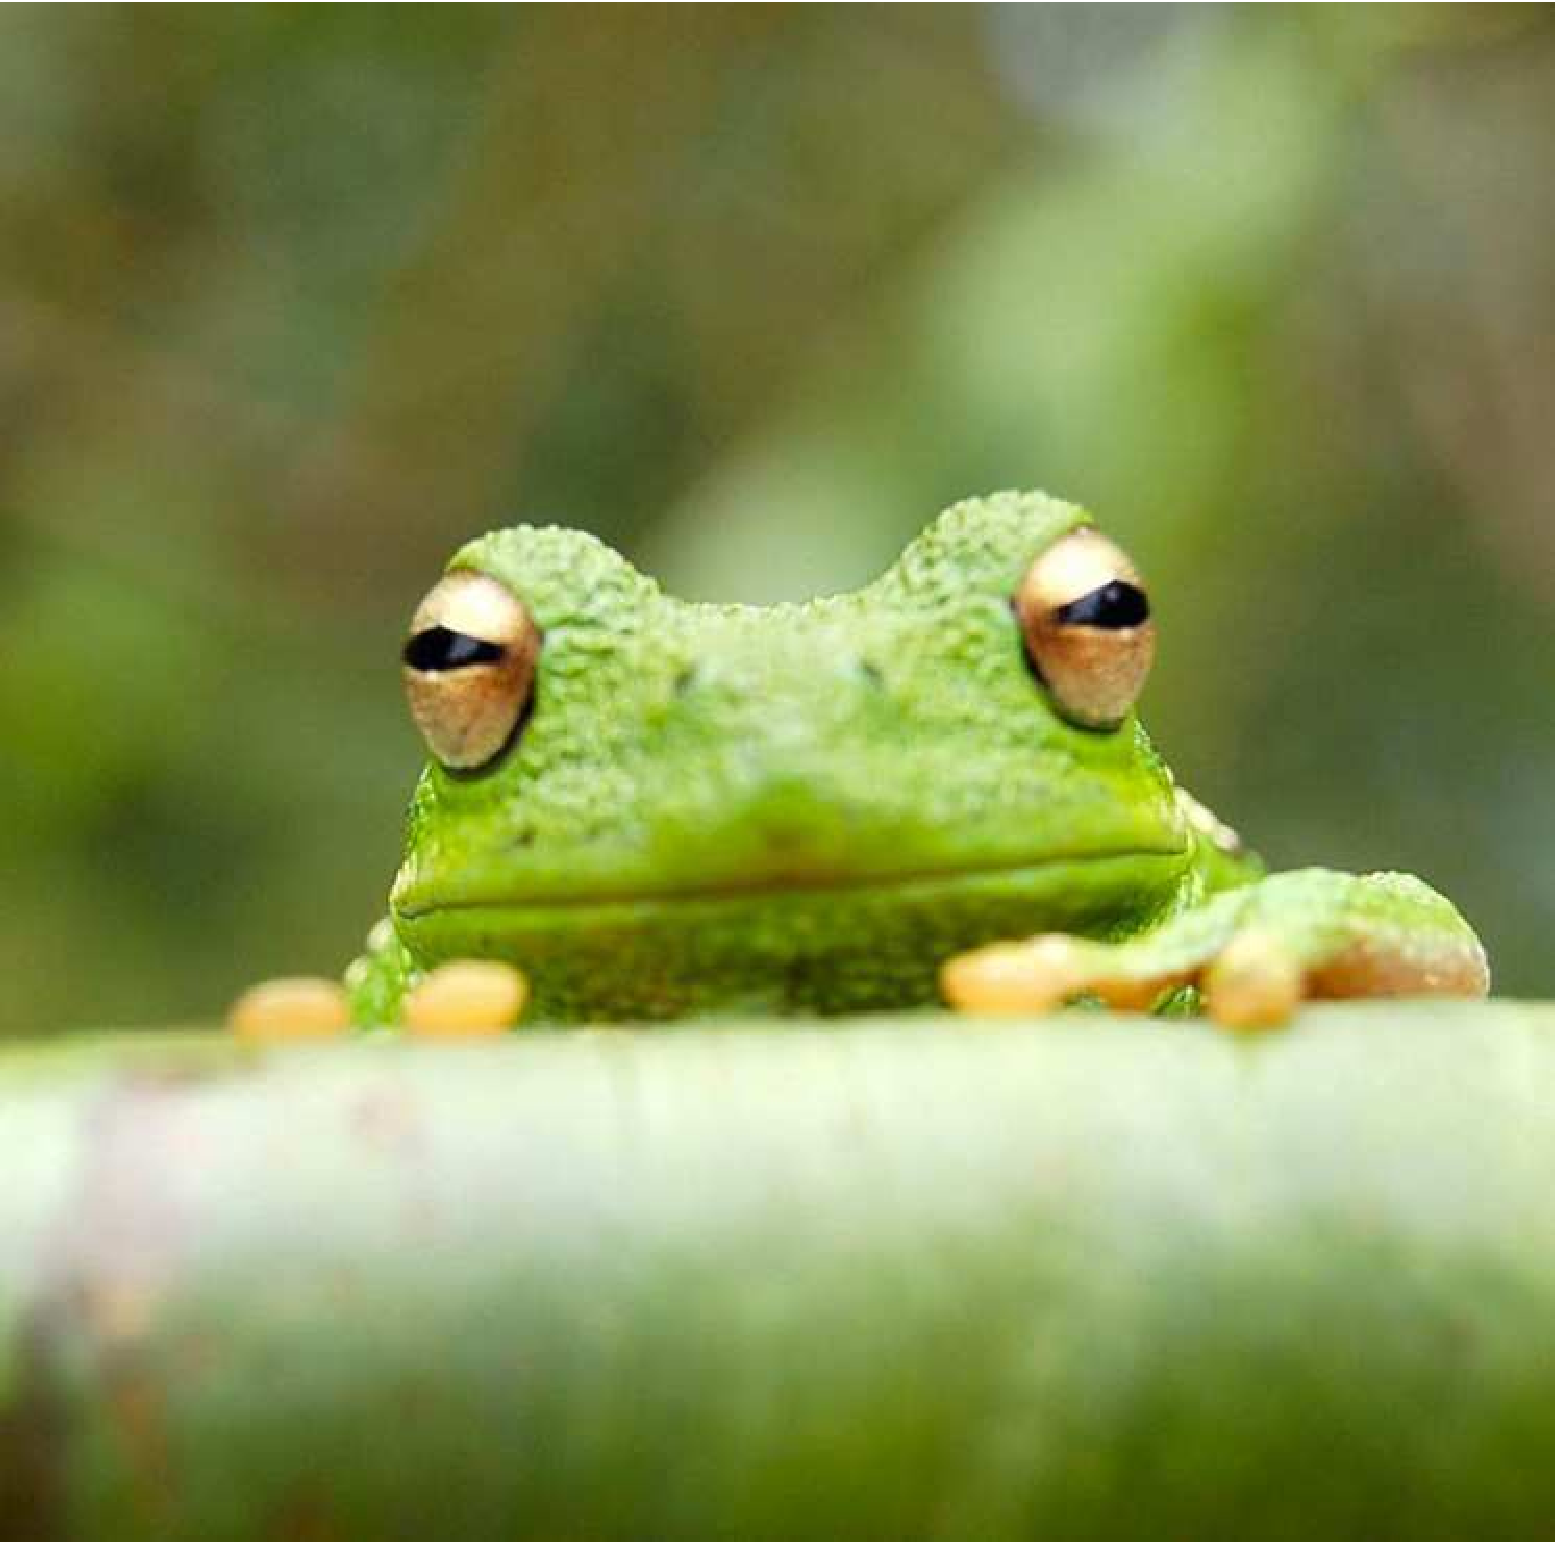
\includegraphics[width=11.4cm,height=11.4cm]{frog.pdf}
\caption{This legend would be placed at the side of the figure, rather than below it.}\label{fig:side}
\end{SCfigure*}


\subsection*{Tables}
Tables should be included in the main manuscript file and should not be uploaded separately.


\subsection*{Footnotes}

Footnotes are ordered by symbols such as *, \textdagger, \textdaggerdbl, etc. The article should contain only 13 footnotes\footnote{Footnote Example 1}\footnote{Footnote Example 2}.


\subsection*{Single column equations}

Authors may use 1- or 2-column equations in their article, according to their preference.

\begin{align*}
(x+y)^3&=(x+y)(x+y)^2\\
       &=(x+y)(x^2+2xy+y^2) \numberthis \label{eqn:example1} \\
       &=x^3+3x^2y+3xy^3+x^3.
\end{align*}

To allow an equation to span both columns, use the \verb|\begin{figure*}...\end{figure*}| environment mentioned above for figures.

Note that the use of the \verb|widetext| environment for equations is not recommended, and should not be used.

\begin{figure*}[bt!]
\begin{align*}
(x+y)^3&=(x+y)(x+y)^2\\
       &=(x+y)(x^2+2xy+y^2) \numberthis \label{eqn:example2} \\
       &=x^3+3x^2y+3xy^3+x^3.
\end{align*}
\end{figure*}



\subsection*{Supporting Information Appendix (SI)}

Authors should submit SI as a single separate SI Appendix PDF file, combining all text, figures, tables, movie legends, and SI references. SI will be published as provided by the authors; it will not be edited or composed. Additional details can be found in the \href{https://www.pnas.org/author-center/submitting-your-manuscript#supporting-information}{PNAS Author Center}. The PNAS Overleaf SI template can be found \href{https://www.overleaf.com/latex/templates/pnas-template-for-supplementary-information/wqfsfqwyjtsd}{here}. Refer to the SI Appendix in the manuscript at an appropriate point in the text. Number supporting figures and tables starting with S1, S2, etc.

Authors who place detailed materials and methods in an SI Appendix must provide sufficient detail in the main text methods to enable a reader to follow the logic of the procedures and results and also must reference the SI methods. If a paper is fundamentally a study of a new method or technique, then the methods must be described completely in the main text.

Supporting information (SI) for PNAS Brief Reports is limited to extended methods, essential supporting datasets, software, and video/audio files; supporting text, tables or figures are not permitted.

\subsubsection*{SI Datasets}

Supply .xlsx, .csv, .txt, .rtf, GZ or .pdf files. This file type will be published in raw format and will not be edited or composed.


\paragraph*{SI Movies}

Supply Audio Video Interleave (avi), Quicktime (mov), Windows Media (wmv), animated GIF (gif), or MPEG-4 Part 14 (mp4) files. Movie legends should be included in the SI Appendix file. All movies should be submitted at the desired reproduction size and length. Movies should be no more than 10MB in size.



\matmethods{Please describe your materials and methods here. This can be more than one paragraph, and may contain subsections and equations as required. If your research involved human or animal participants, please identify the institutional review board and/or licensing committee that approved the experiments. Please also include a brief description of your informed consent procedure if your experiments involved human participants.


\subsection*{Subsection for Method}
Example text for subsection.
}

\showmatmethods{} % Display the Materials and Methods section

\dataavail{To allow others to replicate and build on work published in PNAS, authors must make materials, data, and associated protocols, including code and scripts, available to readers in a public repository upon publication. Restrictions on full or partial access to these materials and requests for legal, ethical, and logistical (e.g., size) exceptions must be noted at submission. If requested, these materials must be made available to editors and reviewers during submission for the purpose of evaluating the manuscript. A statement detailing sharing plans will be included in the published article as provided within the submission form. Research datasets, whether original or previously published, must be cited in the references as a condition for publication. Please refer to our full \href{https://www.pnas.org/author-center/editorial-and-journal-policies\#materials-and-data-availability}{policy}.}

\acknow{Please include your acknowledgments here, set in a single paragraph. Please do not include any acknowledgments in the Supporting Information, or anywhere else in the manuscript.}

\showacknow{} % Display the acknowledgments section




\bibsplit[3]
%Use \bibsplit to split the references from the body of the text. Value "[3]" represents the number of reference in the left column (Note: Please avoid single column figures & tables on this page.)

% Bibliography
\bibliography{pnas-sample}

\end{document}
